%% ym-boundary-mixed-derivative — GitHub edition (pdfTeX / latexmk -pdf)
\documentclass[11pt,a4paper]{article}
\usepackage{lmodern}
\usepackage[T1]{fontenc}
\usepackage[utf8]{inputenc}
\usepackage[a4paper,top=27mm,bottom=27mm,left=28mm,right=28mm]{geometry}
\usepackage{amsmath,amssymb,amsthm}
\usepackage{booktabs}
\usepackage{longtable}
\usepackage{microtype}
\usepackage{enumitem}
\usepackage{graphicx}
\usepackage[hidelinks]{hyperref}
\usepackage{url}

\newtheorem{theorem}{Theorem}[section]
\newtheorem{lemma}[theorem]{Lemma}
\newtheorem{proposition}[theorem]{Proposition}
\newtheorem{corollary}[theorem]{Corollary}
\theoremstyle{definition}
\newtheorem{definition}[theorem]{Definition}
\theoremstyle{remark}
\newtheorem{remark}[theorem]{Remark}

\newcommand{\gb}{\bar g^{2}}
\newcommand{\bR}{\beta_R}
\newcommand{\DR}{D_R}

\title{A boundary observable separating U(1) and SU(2) lattice gauge theory: one loop, a strong-coupling sign and Monte Carlo}
\author{Yoshikazu Hosomura\\[.3em]\normalsize with the assistance of Claude (Claude Code, Anthropic)}
\date{2026-10-29}

\begin{document}
\maketitle
\begin{center}\small wvbks0 [at] gmail.com · \url{https://computoergosum.com/en/index.html}\end{center}
\begin{center}\small AI use is disclosed in \S\ref{sec:ai}; what is not claimed is in \S\ref{sec:notclaimed}.\end{center}

\begin{abstract}
In the Schrödinger functional of four-dimensional lattice gauge theory we separate the boundary angle into a lower angle $\alpha$ and an upper angle $\gamma$, and compare two quantities normalised to equal the bare coupling $\beta$ at tree level: the usual Schrödinger-functional coupling $\bR=4/\gb$, a first derivative at the symmetric point, and $\DR$, a finite-difference version of the mixed derivative $\partial^2\ln Z/\partial\alpha\,\partial\gamma$, which contains no contact term and drops every free energy that depends on one boundary only. We study $h:=\bR-\DR$ in three regimes. At one loop (SU(2), Wilson action, $L/a=4$ to $24$, computed directly on the lattice) the coefficient of $\ln(L/a)$ in $\DR$ equals the predicted $-8b_0$ to within $1\%$, as does that of $\bR$, the constants differ by $0.21$, so that $h\to-0.21$, and the whole difference comes from the charged fluctuations; it is zero in the neutral sector, which suggests (without a separate computation) that it vanishes for U(1). At strong coupling, for fixed $L/a\ge4$ and under the convergence of the polymer expansion, which we take as an assumption, $h<0$ with leading term $-(8/s)u^{3L}$, $s=\sin(\pi/(2L^2))$; the arithmetic and inequality steps of this argument are written in Lean~4 and pass its check. A Monte Carlo study on one laptop (SU(2): 36 points, $L/a=3$ to $8$; U(1): 21 points) gives the shape of $h$ as a function of $\gb$: $h$ turns positive near $\gb\approx4.5$, has a maximum $0.14$ to $0.18$ for $\gb\approx5$ to $10$, returns to zero for $\gb\approx60$ to $120$ and lies between $-0.03$ and $0$ beyond; for $L/a\ge4$ and $\gb\approx35$ to $140$ the lattice sizes agree point by point within about $2\sigma$. In U(1), $h$ is compatible with zero deep in the Coulomb and in the confined phase, and has a peak at the transition whose height does not decrease at $L/a=8$. The status of the paper is computer-assisted, with Lean for the arithmetic steps, and conditional on the assumptions listed in \S\ref{sec:lean}.
\end{abstract}

\section{Introduction}\label{sec:intro}

The question behind this note is the mass-gap problem for four-dimensional Yang--Mills theory (Clay Millennium Problem, statement by Jaffe and Witten~\cite{JW}; the background we use is collected in the book at \url{https://computoergosum.com/en/principia/yang-mills/index.html}). Nothing here addresses that problem directly. What we look for is a single, well-defined lattice observable whose shape as a function of the renormalised coupling separates the non-abelian theory from compact U(1), which has a massless Coulomb phase. The Schrödinger-functional (SF) coupling of Lüscher, Narayanan, Weisz and Wolff~\cite{LNWW} and of Lüscher, Sommer, Weisz and Wolff~\cite{LSWW} is such an observable in the weak-coupling region, but it is a first derivative with respect to a boundary angle that moves both boundaries at once. In the strong-coupling region the SF coupling therefore picks up free-energy contributions that live at one boundary only (in the strong-coupling expansion, strips of plaquettes winding around one boundary), and these are not related to the propagation of flux between the two boundaries.

We replace the first derivative by the mixed second derivative with respect to the two boundary angles. The idea is elementary: if $\Gamma=-\ln Z$ is written as $f(\alpha)+f(\gamma)+g(\alpha,\gamma)$, the mixed derivative kills $f$ exactly and measures only $g$. This note records, for the difference $h=\bR-\DR$ between the usual SF coupling and the mixed-derivative quantity, what we found in three regimes:
\begin{enumerate}[leftmargin=2em]
\item a one-loop computation on the lattice (\S\ref{sec:oneloop});
\item the sign of $h$ in the strong-coupling expansion, at fixed $L/a\ge4$, with the arithmetic steps written in Lean~4 (\S\ref{sec:strong});
\item a Monte Carlo study of $h$ as a function of $\gb=4/\bR$ for SU(2), and of $h$ for U(1) as a control (\S\ref{sec:mc}).
\end{enumerate}
The SF coupling itself, its one-loop coefficient and the renormalisability argument are from~\cite{LNWW,LSWW}; we reproduce the one-loop coefficient table of~\cite{LNWW} as a check of our code. The use of the mixed derivative as a separate observable, and the numbers below, are what this note adds; we do not know whether the same observable has been studied before. Numbers quoted without a citation are taken from the authors' working records (programs, outputs and reports), which are not published.

\paragraph{Status of the results.} Computer-assisted (floating-point one-loop and Monte Carlo, not interval arithmetic), with the arithmetic and inequality steps of the strong-coupling sign in Lean~4; the strong-coupling statement is conditional on the convergence of the polymer expansion and on the coefficients of the leading terms, which are derived by hand. No statement of this note is an unconditional theorem about the continuum theory.

\section{Setting and definitions}\label{sec:setting}

\subsection{The Schrödinger functional with two boundary angles}

We use the SF of~\cite{LNWW,LSWW} for gauge group SU(2): an $L^3\times L$ lattice (lattice units, $a=1$), periodic in the three spatial directions, with Dirichlet boundary conditions at $x^0=0$ and $x^0=L$, the Wilson action $S=\beta\sum_p w(p)\,(1-\tfrac12\operatorname{tr}U_p)$ with weight $\tfrac12$ on the spatial plaquettes of the two boundaries and $c_t=1$ (no $O(a)$ boundary improvement), and $\beta=4/g_0^2$. The spatial links at $x^0=0$ are $\exp\{(\alpha/L)\,\tau\}$ and those at $x^0=L$ are $\exp\{(\gamma/L)\,\tau\}$, with $\tau$ the fixed Cartan generator, so that the holonomies around a spatial cycle are $W_0=e^{\alpha\tau}$ and $W_L=e^{\gamma\tau}$. The usual SF is $\alpha=\eta$, $\gamma=\pi-\eta$~\cite[(2.5),(2.6)]{LSWW}. The induced classical field is a constant colour-electric field depending on $\gamma-\alpha$ only, and the classical action~\cite[(2.11)]{LSWW}, rewritten for two angles, is
\begin{equation}\label{eq:Scl}
S_{\rm cl}=3\beta L^4\bigl(1-\cos((\gamma-\alpha)/L^2)\bigr).
\end{equation}
For U(1) we use the same geometry and the same normalising formulas (so that at tree level all quantities below equal $\beta$), with $\gb:=1/\bR$.

Let $\Gamma(\alpha,\gamma)=-\ln Z(\alpha,\gamma)$.

\begin{definition}[the two observables]\label{def:obs}
\begin{enumerate}[label=(\roman*),leftmargin=2em]
\item The SF coupling at $\eta=\pi/4$: with $\alpha=\eta$, $\gamma=\pi-\eta$, so that $\partial_\eta=\partial_\alpha-\partial_\gamma$,
\[
\bR:=\frac{\langle\partial_\alpha S-\partial_\gamma S\rangle}{-6L^2\sin(\pi/(2L^2))}\qquad(\alpha=\pi/4,\ \gamma=3\pi/4),
\]
equal to $\beta$ at tree level by~\eqref{eq:Scl}; $\gb:=4/\bR$ for SU(2).
\item The mixed-derivative quantity: with $\alpha=\pi/4$ fixed and $\gamma_1=\pi/2$, $\gamma_2=\pi$,
\[
D:=\frac{\langle\partial_\alpha S\rangle_{\gamma_1}-\langle\partial_\alpha S\rangle_{\gamma_2}}{\gamma_2-\gamma_1}
=\frac{1}{\gamma_2-\gamma_1}\int_{\gamma_1}^{\gamma_2}\frac{\partial^2\ln Z}{\partial\alpha\,\partial\gamma}\,d\gamma ,
\qquad \DR:=\frac{D}{\hat D},
\]
where $\hat D$ is the tree-level value of $D$ at $\beta=1$, so that $\DR=\beta$ at tree level; $0<\hat D\le3$.
\item The normalised mixed derivative at a point: $M_R(\alpha,\gamma):=\bigl(\partial^2\ln Z/\partial\alpha\,\partial\gamma\bigr)/M_{\rm cl}$, where $M_{\rm cl}=3\cos((\gamma-\alpha)/L^2)$ is its tree-level value at $\beta=1$ (from~\eqref{eq:Scl}); unless stated otherwise $M_R$ is taken at the symmetric point $(\pi/4,3\pi/4)$.
\item $h:=\bR-\DR$.
\end{enumerate}
\end{definition}

The equality in (ii) holds because $\partial_\alpha\ln Z=-\langle\partial_\alpha S\rangle$. In the Monte Carlo, $D$ is obtained from two independent runs, one at $\gamma_1$ and one at $\gamma_2$, measuring only $\partial_\alpha S$; this has a statistical error two to six times smaller than the covariance estimator $\langle\partial_\alpha S\,\partial_\gamma S\rangle-\langle\partial_\alpha S\rangle\langle\partial_\gamma S\rangle$ of the same derivative.

\begin{lemma}[no contact term; one-sided terms drop out]\label{lem:mixed}
$\partial^2 S/\partial\alpha\,\partial\gamma=0$, so $\partial^2\ln Z/\partial\alpha\,\partial\gamma=\langle\partial_\alpha S\,\partial_\gamma S\rangle-\langle\partial_\alpha S\rangle\langle\partial_\gamma S\rangle$. If $\Gamma=f_1(\alpha)+f_2(\gamma)+g(\alpha,\gamma)$ then $\partial_\alpha\partial_\gamma\Gamma=\partial_\alpha\partial_\gamma g$.
\end{lemma}
\begin{proof}
$\alpha$ enters $S$ only through the plaquettes touching the lower boundary and $\gamma$ only through those touching the upper boundary; for $L\ge2$ no plaquette touches both. The rest is differentiation under the integral sign (the integrand is smooth and the group compact) and the vanishing of $\partial_\alpha\partial_\gamma$ on functions of one variable.
\end{proof}

By contrast, $\bR$ contains $f_1'(\pi/4)-f_2'(3\pi/4)$. This is the whole reason for introducing $\DR$: $h$ measures, roughly, how much of $\bR$ is carried by one-boundary terms and by the non-trivial dependence of $g$ on $(\alpha,\gamma)$ beyond $\gamma-\alpha$.

\section{One loop}\label{sec:oneloop}

\subsection{What is cited and what is computed}

At one loop $\Gamma=\beta s_0+\Gamma_1+O(1/\beta)$ with $s_0=S_{\rm cl}/\beta$. With $\beta=\beta(\mu)-8b_0\ln(a\mu)$, $8b_0=11/(3\pi^2)=0.37151$ for SU(2), finiteness of $\Gamma$ requires
\[
\Gamma_1(\alpha,\gamma)=-8b_0\ln(L/a)\,s_0(\gamma-\alpha)+F(\alpha,\gamma)+O(a/L).
\]
That the logarithm multiplies $s_0$ and that no other logarithmic (boundary) counterterm appears is the renormalisability statement of~\cite{LNWW}: the Seeley--DeWitt coefficient that produces the pole is a volume integral of $\operatorname{tr}G_{\mu\nu}G_{\mu\nu}$ and has no boundary term~\cite[(3.28), (3.36)]{LNWW}. It follows by hand that $\bR$ and $\DR$ have the same one-loop logarithm $-8b_0\ln(L/a)$, i.e.\ the same one-loop step $8b_0\ln2=0.2575$ under $L\to2L$, while the constants
\[
\bR=\beta-8b_0\ln(L/a)+c_\eta+\dots,\qquad \DR=\beta-8b_0\ln(L/a)+c_D+\dots
\]
may differ, because $F$ is not a function of $\gamma-\alpha$ alone. Indeed the background field strength depends only on $\gamma-\alpha$, but the constant part $\alpha/L$ of the spatial background is a holonomy $e^{2i\alpha}$ seen by the charged fluctuations, which cannot be gauged away.

We computed $\Gamma_1(\alpha,\gamma)$ directly on the lattice: the second variation of the SU(2) Wilson action around the SF background, without any further approximation of the action, the ghost operator on $1\le x^0\le L-1$ together with the constant boundary mode of~\cite[(6.3)]{LNWW}, and $\Gamma_1=\tfrac12\ln\det(H+\lambda DD^\dagger)-\ln\det(D^\dagger D)$, decomposed into charge sectors and spatial momenta; derivatives in $\alpha,\gamma$ by a nine-point stencil with Richardson extrapolation. As a check, the one-loop coefficient $m_1(L)=-\bR^{(1)}/4$ of the SF coupling agrees with Table~1 of~\cite{LNWW} to eight digits for $L/a=6,8,10,12,16,20,24$ (for example $0.35422030$, $0.45347745$, $0.49316916$). Further checks: gradient of the action at the background $3\times10^{-17}$; $|HD|\le10^{-15}$ (the kernel of the Hessian is the gauge orbit); dependence on the gauge parameter $\lambda$ only through the constant $\tfrac12 n_g\ln\lambda$.

\subsection{Results}

Table~\ref{tab:oneloop} lists the one-loop coefficients (the part of each quantity proportional to $\beta^0$, in units where the tree level is $\beta$). $M_R^{(1)}$ is the mixed derivative at the symmetric point $(\pi/4,3\pi/4)$, $\DR^{(1)}$ the average over $\gamma\in[\pi/2,\pi]$ used in the Monte Carlo.

\begin{table}[ht]\centering\footnotesize\setlength{\tabcolsep}{3.5pt}
\caption{One-loop coefficients on the lattice, SU(2), Wilson action, $c_t=1$.}\label{tab:oneloop}
\begin{tabular}{@{}rrrrrrr@{}}\toprule
$L/a$ & $M_R^{(1)}$ & $\DR^{(1)}$ & $\bR^{(1)}=-4m_1$ & $\bR^{(1)}-\DR^{(1)}$ & neutral $M_R^{(1)}$ & charged $M_R^{(1)}$\\\midrule
4 & $-0.93558$ & $-0.94624$ & $-1.25205$ & $-0.3058$ & $-0.2349$ & $-0.7007$\\
6 & $-1.17123$ & $-1.17290$ & $-1.41688$ & $-0.2440$ & $-0.2386$ & $-0.9326$\\
8 & $-1.30854$ & $-1.30779$ & $-1.53482$ & $-0.2270$ & $-0.2412$ & $-1.0673$\\
10 & $-1.40695$ & $-1.40524$ & $-1.62577$ & $-0.2205$ & $-0.2429$ & $-1.1640$\\
12 & $-1.48425$ & $-1.48205$ & $-1.69932$ & $-0.2173$ & $-0.2441$ & $-1.2402$\\
16 & $-1.60239$ & $-1.59973$ & $-1.81391$ & $-0.2142$ & $-0.2455$ & $-1.3568$\\
20 & $-1.69172$ & $-1.68885$ & $-1.90164$ & $-0.2128$ & $-0.2464$ & $-1.4453$\\
24 & $-1.76361$ & $-1.76064$ & $-1.97268$ & $-0.2120$ & $-0.2470$ & $-1.5166$\\\bottomrule
\end{tabular}
\end{table}

Fitting $b\ln N+c+d/N+e/N^2$ ($N=L/a\ge8$):
\begin{itemize}[leftmargin=2em]
\item free $b$: $M_R^{(1)}$ gives $b=-0.37488$, which is $1.009$ times $-8b_0$; $\DR^{(1)}$ gives $-0.37432$ ($1.008$ times); $\bR^{(1)}$ gives $-0.36979$ ($0.995$ times); the free $b$ of $M_R^{(1)}$ moves by $1$--$3\%$ with the fit range;
\item $b$ fixed at $-8b_0$: $c_M=-0.600(3)$, $c_D=-0.598(3)$, $c_\eta=-0.8099$, the last to be compared with $-4r_0=-0.8094$ from~\cite[(7.39)]{LNWW}; the errors are the spread over fit ranges and forms, not statistical;
\item the difference $\bR^{(1)}-M_R^{(1)}$ has a fitted logarithmic coefficient $+0.0051$, compatible with zero, and tends to $-0.21$.
\end{itemize}
The doubling steps of $M_R^{(1)}$ are $0.373$, $0.294$, $0.279$ for $4\to8$, $8\to16$, $12\to24$, approaching $0.2575$ from above (those of $\bR^{(1)}$ are $0.283$, $0.279$, $0.273$).

\paragraph{Charged and neutral sectors.} The neutral sector contributes a constant ($M_R^{(1)}\to-0.247$) with no logarithm, and contributes nothing to the difference: the neutral part of $\bR^{(1)}-M_R^{(1)}$ is $+0.00186$, $+0.00012$, $+0.00001$, $0.00000$ at $L/a=4,8,16,24$, while the charged part is $-0.31833$, $-0.22639$, $-0.21153$, $-0.20907$. In the neutral sector $F$ is a function of $\gamma-\alpha$ only (we checked $\partial_\alpha^2\Gamma_1=-\partial_\alpha\partial_\gamma\Gamma_1$ there to $10^{-8}$), whereas the charged sector gives $(\partial_\alpha^2+\partial_\alpha\partial_\gamma)\Gamma_1=-2.07$ at $L/a=24$. U(1) has no charged fluctuations, so in this normalisation its one-loop $h$ is zero; this is a reading of the neutral-sector computation, not a separate U(1) computation.

\paragraph{The edge $\gamma=\pi$.} The upper angle $\gamma=\pi$ lies on the edge of the fundamental domain of~\cite[(5.8)]{LNWW}: the upper holonomy is central and two charged zero modes appear, with lowest eigenvalue proportional to $\pi-\gamma$, so $-\partial_\gamma^2\Gamma_1\approx1/(\pi-\gamma)^2$ (we find $994$, $995$, $996$ at $\gamma=0.99\pi$ for $L/a=4,8,16$, against $1/(0.01\pi)^2=1013$). The mixed derivative stays finite and smooth: $M_R^{(1)}(\pi/4,\gamma)$ varies by $2.5\%$ over $\gamma\in[\pi/2,0.99\pi]$ at $L/a=16$. For $\DR^{(1)}$ the value at $\gamma_2=\pi$ is a linear extrapolation from $\pi-0.01$ and $\pi-0.003$; replacing $\gamma_2$ by $7\pi/8$ changes $\DR^{(1)}$ by less than $0.004$ at $L/a=24$.

\paragraph{Summary of the weak-coupling end.} $\DR$ and $\bR$ have the same one-loop running; $h\to-0.21$ at one loop, with the sign $\DR>\bR$; all of it comes from charged fluctuations.

\section{Strong coupling}\label{sec:strong}

Let $u=I_2(\beta)/I_1(\beta)$ be the fundamental character coefficient of the SU(2) Wilson action ($u\approx\beta/4$ for small $\beta$). The spatial boundary plaquettes are trivial, so contractible surfaces do not depend on $\alpha,\gamma$; only surfaces bounded by loops winding around a spatial cycle at a boundary do. Two families give the lowest orders (counted by hand):
\begin{itemize}[leftmargin=2em]
\item one-sided strips (a winding loop at one boundary, closed by a U-shaped strip of area $3L$): $6L^2$ positions per boundary, each with weight $u^{3L}\chi(W)^2$, giving $\ln Z\supset B(\cos^2\alpha+\cos^2\gamma)$, $B=24L^2u^{3L}$;
\item cylinders joining the two boundaries (area $L^2$, and with one step, area $L^2+L$): $\ln Z\supset A\cos\alpha\cos\gamma$, $A=12L^2u^{L^2}\bigl(1+4(L-1)u^L\bigr)$.
\end{itemize}
The strips enter $\bR$ and, by Lemma~\ref{lem:mixed}, not $\DR$. With $s=\sin(\pi/(2L^2))$ their contribution is $\bR\supset-2B/(6L^2s)=-(8/s)u^{3L}$, and $8/s\ge16L^2/\pi$. The cylinders contribute $A/(6L^2s)$ to $\bR$ and $A\sqrt2/(\pi\hat D)$ to $\DR$, so their contribution to $h$ is $\bigl(1/(6L^2s)-\sqrt2/(\pi\hat D)\bigr)A$, whose coefficient is negative for $L\ge4$. Both contributions have the same sign. Since $u^{L^2}\le u^{3L}u^L$ for $L\ge4$ and $0\le u\le1$, the cylinder term is of higher order than the strip term.

\begin{proposition}[conditional]\label{prop:strong}
Fix $L\ge4$. Assume (H): the remainder $R$ of $h$ beyond the strip and cylinder terms satisfies $|R|\le C_Lu^{3L+1}$ for $0<u\le u_0$, with some $u_0>0$ and $C_L\ge0$. Then, with $K=8/s$ and $G=\bigl(1/(6L^2s)-\sqrt2/(\pi\hat D)\bigr)A\le0$,
\[
h=-K u^{3L}+G+R,\qquad |h-(-Ku^{3L}+G)|\le C_Lu\cdot u^{3L},
\]
and $h<0$ for every $u\in(0,\min(u_0,u_1)]$, where $u_1>0$ is any number with $C_Lu_1<K$, i.e.\ for all $\beta$ below some $\beta_0(L)>0$.
\end{proposition}

\begin{proof}[Structure of the proof]
The expansion of $\ln Z$ into the strip, cylinder and remainder terms and the coefficients $B$, $A$ are derived by hand; (H) is what one expects from the convergence of the polymer (cluster) expansion of Osterwalder and Seiler~\cite{OS}, but we have not derived it for this boundary geometry and use it as an assumption. Given these, the steps are: $3L+L\le L^2$ for $L\ge4$; $u^{L^2}\le u^{3L}u^L$; $-2(24L^2u^n)/(6L^2s)=-(8/s)u^n$; $8/s\ge16L^2/\pi$ when $0<s\le\pi/(2L^2)$ (i.e.\ $\sin x\le x$); $1/(6L^2s)<\sqrt2/(\pi\hat D)$ for $L\ge4$, $0<\hat D\le3$ and $s>x-x^3/4$ with $x=\pi/(2L^2)$; non-positivity of the cylinder part $G$, using $A\ge0$; the bound on $|h-(-Ku^{3L}+G)|$ from (H) (in Lean stated for $-Ku^{3L}+R$, which is the same inequality since $G$ cancels); and $h<0$ when $C_Lu<K$, then on the whole interval $(0,\min(u_0,u_1)]$, by applying \texttt{h\_neg\_on\_interval} with $u_0$ replaced by $\min(u_0,u_1)$. Each of these is a theorem of the Lean file described in \S\ref{sec:lean} (Table~\ref{tab:corr}), stated for abstract real numbers $K$, $C$, $G$, $R$; the inequalities $\sin x\le x$ and $\sin x>x-x^3/4$, the bounds $\hat D\le3$ and $A\ge0$, and (H) enter as hypotheses.
\end{proof}

We do not evaluate $C_L$ or $u_0$, and we do not claim a $\beta_0$ uniform in $L$ (the count of folded strips grows with $L$). For $L=3$ one has $3L=L^2$ and for $L\le3$ the cylinder is leading, so this statement says nothing about the Monte Carlo points at $L/a=3$, which in any case lie outside the range $L/a\ge4$ required in~\cite[(2.9)]{LSWW}. Nor does it say anything about $\beta\ge2$, where the leading strong-coupling terms are below $10^{-3}$ and the measured values are of order $10^{-1}$.

\section{Monte Carlo}\label{sec:mc}

\subsection{Setup}

Heat-bath updates followed by overrelaxation sweeps (one overrelaxation per heat bath for $L/a\le4$, two for $L/a\ge6$); thermalisation $200$ sweeps ($500$ for $L/a=3$, $300$ for $L/a=10$, $400$ in the last U(1) series); one measurement per update cycle. For $\DR$ we used, from the second series on, the one-link integral at $x^0=1$: each term of $\partial_\alpha S$ is linear in one link at $x^0=1$ whose other factors do not contain it, so the link can be replaced by its conditional expectation without changing the expectation value. This reduces the variance by a factor $1.6$ to $1.8$; plain and one-link estimates agree within errors at every point where both were taken. $\bR$ comes from separate runs at $(\pi/4,3\pi/4)$. Errors are binned jackknife errors, taking the largest over bin widths $25,50,100,200$; errors of $\bR$ and $\DR$, which come from independent runs, are added in quadrature. Each run used one core of one laptop computer. The numbers of measurements per run are summarised in Table~\ref{tab:stats}; where several series exist at one point, the table of results uses their error-weighted mean.

\begin{table}[ht]\centering\small
\caption{Monte Carlo series and measurements per run (one run per value of $\gamma$; $\DR$ needs two runs, $\bR$ one).}\label{tab:stats}
\begin{tabular}{@{}lp{0.45\linewidth}p{0.30\linewidth}@{}}\toprule
Series & Points & Measurements per run\\\midrule
first & SU(2), U(1), $L/a\le8$ & 2000 (1500 at $L/a=8$; one run 1250)\\
second & SU(2) $\beta=1.6$--$2.5$, $L/a=3$--$10$; U(1) & 6000--10000\\
third & SU(2) $\beta=1.6$--$2.3$, $L/a=3$--$8$ & 5000--10000\\
fourth & SU(2) near $h=0$ and the maximum, $L/a=4,6,8$ & 8000--96000\\
fifth & U(1) $\beta=0.8$--$1.3$, $L/a=4,6,8$ & 16000--24000\\\bottomrule
\end{tabular}
\end{table}

\subsection{SU(2)}

Table~\ref{tab:su2} and Figure~\ref{fig:h}(a) give all 36 SU(2) points. For the points with $\bR\lesssim0.04$ the relative error of $\bR$ is large and enters $\gb=4/\bR$ directly; at three points ($L/a=3$, $\beta=1.6$; $L/a=8$, $\beta=2.28$ and $2.20$) $\bR$ is compatible with zero, so their $\gb$ is not determined (only bounded below).

\begin{table}[tp]\centering\small
\caption{SU(2): $\bR$, $\DR$ and $h=\bR-\DR$ (combined series).}\label{tab:su2}
\begin{tabular}{@{}rrrlll@{}}\toprule
$L/a$ & $\beta$ & $\gb$ & $\bR$ & $\DR$ & $h$\\\midrule
3 & 2.20 & 5.53 & 0.7228(80) & 0.5439(182) & $+0.179(20)$\\
3 & 2.00 & 12.8 & 0.3134(88) & 0.1907(158) & $+0.123(18)$\\
3 & 1.90 & 23.9 & 0.1671(77) & 0.1308(107) & $+0.036(13)$\\
3 & 1.80 & 61.9 & 0.0647(51) & 0.0690(94) & $-0.004(11)$\\
3 & 1.70 & 258 & 0.0155(43) & 0.0479(84) & $-0.032(9)$\\
3 & 1.60 & 1017 & 0.0039(44) & 0.0332(67) & $-0.029(8)$\\\midrule
4 & 2.70 & 3.29 & 1.2142(123) & 1.3065(539) & $-0.092(55)$\\
4 & 2.40 & 4.83 & 0.8276(196) & 0.8111(792) & $+0.017(82)$\\
4 & 2.30 & 6.15 & 0.6505(104) & 0.5068(291) & $+0.144(31)$\\
4 & 2.20 & 10.4 & 0.3834(230) & 0.2203(218) & $+0.163(32)$\\
4 & 2.15 & 13.7 & 0.2920(116) & 0.1853(209) & $+0.107(24)$\\
4 & 2.10 & 22.5 & 0.1775(54) & 0.0804(79) & $+0.097(10)$\\
4 & 2.05 & 46.4 & 0.0862(46) & 0.0796(72) & $+0.007(8)$\\
4 & 2.00 & 105 & 0.0379(36) & 0.0527(57) & $-0.015(7)$\\
4 & 1.95 & 534 & 0.0075(32) & 0.0345(56) & $-0.027(6)$\\\midrule
6 & 2.40 & 8.13 & 0.4923(224) & 0.3171(377) & $+0.175(44)$\\
6 & 2.35 & 11.4 & 0.3519(170) & 0.1973(341) & $+0.155(38)$\\
6 & 2.30 & 16.6 & 0.2407(139) & 0.1150(228) & $+0.126(27)$\\
6 & 2.28 & 25.4 & 0.1575(109) & 0.1017(181) & $+0.056(21)$\\
6 & 2.27 & 30.0 & 0.1334(106) & 0.1096(185) & $+0.024(21)$\\
6 & 2.26 & 33.2 & 0.1205(58) & 0.0623(99) & $+0.058(12)$\\
6 & 2.25 & 38.5 & 0.1040(64) & 0.0833(109) & $+0.021(13)$\\
6 & 2.22 & 78.4 & 0.0510(58) & 0.0511(94) & $-0.000(11)$\\
6 & 2.20 & 168 & 0.0239(52) & 0.0316(90) & $-0.008(10)$\\\midrule
8 & 2.70 & 4.79 & 0.8355(127) & 0.8575(282) & $-0.022(31)$\\
8 & 2.60 & 5.76 & 0.6944(148) & 0.5741(325) & $+0.120(36)$\\
8 & 2.50 & 7.92 & 0.5052(121) & 0.3676(258) & $+0.138(29)$\\
8 & 2.40 & 18.6 & 0.2147(391) & 0.0983(375) & $+0.117(54)$\\
8 & 2.36 & 34.0 & 0.1176(92) & 0.0737(150) & $+0.044(18)$\\
8 & 2.35 & 43.3 & 0.0924(53) & 0.0556(100) & $+0.037(11)$\\
8 & 2.34 & 65.8 & 0.0608(52) & 0.0373(100) & $+0.024(11)$\\
8 & 2.32 & 105 & 0.0382(66) & 0.0325(127) & $+0.006(14)$\\
8 & 2.33 & 124 & 0.0323(112) & 0.0354(195) & $-0.003(23)$\\
8 & 2.28 & 198 & 0.0202(153) & 0.0194(291) & $+0.001(33)$\\
8 & 2.30 & 315 & 0.0127(62) & 0.0439(111) & $-0.031(13)$\\
8 & 2.20 & 980 & 0.0041(252) & 0.0112(234) & $-0.007(34)$\\\bottomrule
\end{tabular}
\end{table}

\begin{figure}[ht]\centering
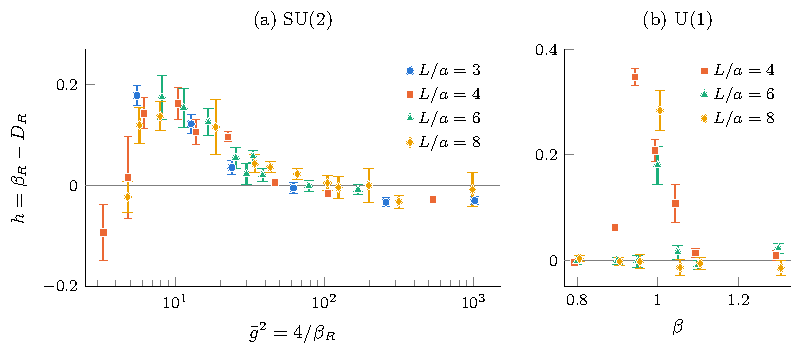
\includegraphics[width=\linewidth]{fig-h.pdf}
\caption{(a) SU(2): $h=\bR-\DR$ against $\gb=4/\bR$ (logarithmic axis), by lattice size. (b) U(1): $h$ against $\beta$; the points of the three lattice sizes are shifted by $\pm0.006$ in $\beta$ for legibility. Data: Tables~\ref{tab:su2} and~\ref{tab:u1}.}\label{fig:h}
\end{figure}

\paragraph{Shape.} Read from the table:
\begin{itemize}[leftmargin=2em]
\item near $\gb\approx4.5$, $h$ is compatible with zero ($L/a=4$: $+0.017(82)$ at $4.8$; $L/a=8$: $-0.022(31)$ at $4.8$), and the only point below, $L/a=4$ at $\gb=3.3$, has $-0.092(55)$, on the side of the one-loop value $-0.21$;
\item the maximum lies at $\gb\approx5$ to $10$ with height $0.14$ to $0.18$ ($L/a=3$: $0.179(20)$ at $5.5$; $L/a=4$: $0.163(32)$ at $10.4$; $L/a=6$: $0.175(44)$ at $8.1$; $L/a=8$: $0.138(29)$ at $7.9$); the differences between these four maxima are $0.1$ to $1.2\sigma$;
\item $h$ decreases to $0.02$--$0.10$ for $\gb\approx20$ to $40$ and reaches zero for $\gb\approx60$ to $120$: by linear interpolation between neighbouring points in $\gb$, $57.8$ ($L/a=3$), $64.4$ ($L/a=4$), $78.2$ ($L/a=6$, where one point is $0.000(11)$) and $117$ ($L/a=8$);
\item beyond $\gb\approx150$, $h$ lies between $-0.03$ and $0$.
\end{itemize}
For $L/a\ge4$ and $\gb\approx35$ to $140$, points of different lattice sizes at comparable $\gb$ agree within about $2\sigma$ (the largest difference is $2.1\sigma$, between $L/a=8$ at $\gb=43.3$ and $L/a=4$ at $46.4$); with comparable statistics at $L/a=4$, $6$ and $8$, no systematic excess of $L/a=8$ remains there. Outside this range the agreement is not uniform: $L/a=3$ at $\gb=23.9$ ($+0.036(13)$) and $L/a=4$ at $22.5$ ($+0.097(10)$) differ by $3.8\sigma$. The order $58<64<78<117$ of the zero crossings is suggestive of a drift with $L$, but no pair of points at the same $\gb$ differs by $2\sigma$ in that region, and the $\gb$ values there are poorly determined. We therefore regard the right-edge $L$-dependence as undecided.

\paragraph{Comparison with one loop in the renormalised coupling.} Taking the measured $\bR$ as input and the lattice one-loop difference $\Delta(N)=\DR^{(1)}-\bR^{(1)}$ (Table~\ref{tab:oneloop}), the prediction $\DR\approx\bR+\Delta(N)$ exceeds the measured $\DR$ at the five weak-coupling points of Table~\ref{tab:su2} ($\beta=2.7$ and $2.4$) by $\delta=0.205(31)$ to $0.419(44)$. At the three points with $\gb\le4.83$, $\delta\cdot\bR$ is $0.259(67)$, $0.171(26)$ and $0.267(68)$, roughly $0.17$ to $0.27$ (weighted mean $0.19(2)$, $\chi^2=2.9$ for two degrees of freedom); a term $\delta\propto\gb$ of this size is consistent with a next-order (two-loop) correction, but three points do not determine its coefficient. At $\gb=8.1$ and $18.6$, $\delta\cdot\bR$ is $0.206(24)$ and $0.074(18)$. We did not compute two loops.

\subsection{U(1)}

\begin{table}[ht]\centering\small
\caption{U(1): $\bR$, $\DR$ and $h$ (normalised as for SU(2), tree level $=\beta$).}\label{tab:u1}
\begin{tabular}{@{}rlllllllll@{}}\toprule
 & \multicolumn{3}{c}{$L/a=4$} & \multicolumn{3}{c}{$L/a=6$} & \multicolumn{3}{c}{$L/a=8$}\\
$\beta$ & $\bR$ & $\DR$ & $h$ & $\bR$ & $\DR$ & $h$ & $\bR$ & $\DR$ & $h$\\\midrule
0.80 & 0.003 & 0.007 & $-0.004(4)$ & $-0.001$ & 0.001 & $-0.002(5)$ & $-0.001$ & $-0.005$ & $+0.003(5)$\\
0.90 & 0.051 & $-0.012$ & $+0.063(8)$ & $-0.000$ & 0.000 & $-0.001(7)$ & $-0.004$ & $-0.002$ & $-0.002(8)$\\
0.95 & 0.353 & 0.005 & $+0.348(16)$ & 0.008 & 0.009 & $-0.002(11)$ & 0.002 & 0.004 & $-0.002(14)$\\
1.00 & 0.579 & 0.371 & $+0.208(21)$ & 0.508 & 0.327 & $+0.181(36)$ & 0.443 & 0.159 & $+0.285(38)$\\
1.05 & 0.670 & 0.562 & $+0.108(36)$ & 0.669 & 0.653 & $+0.015(13)$ & 0.659 & 0.673 & $-0.013(16)$\\
1.10 & 0.764 & 0.750 & $+0.014(8)$ & 0.748 & 0.756 & $-0.009(9)$ & 0.740 & 0.745 & $-0.006(12)$\\
1.30 & 1.006 & 0.996 & $+0.010(10)$ & 1.002 & 0.979 & $+0.023(10)$ & 0.980 & 0.994 & $-0.014(14)$\\\bottomrule
\end{tabular}
\end{table}

Table~\ref{tab:u1} and Figure~\ref{fig:h}(b). Deep in the Coulomb phase ($\beta=1.1$, $1.3$) and in the confined phase ($\beta=0.8$, and $0.9$, $0.95$ for $L/a\ge6$), $h$ is compatible with zero (largest deviation $2.2\sigma$). In the Coulomb phase $\DR$ is compatible with a constant in $L$ (for example $0.750(8)$, $0.756(8)$, $0.745(11)$ at $\beta=1.1$), as expected from the free photon, while $\bR$ decreases slightly with $L$ (about $-0.025$ from $L/a=4$ to $8$, $4$ to $5\sigma$). At the transition $h$ has a peak: at $L/a=4$ it spans $\beta=0.90$ to $1.05$ (maximum $0.348(16)$ at $0.95$, where $\bR$ has risen to $0.35$ and $\DR$ is still zero); at $L/a=6$ and $8$ only the point $\beta=1.00$ is non-zero, $0.181(36)$ and $0.285(38)$. The width shrinks below the $\beta$ spacing $0.05$ of our scan, but the height at $\beta=1.00$ does not decrease from $L/a=6$ to $8$. The $L/a=6$ run at $\beta=1.00$ had not settled (block averages drifting over the first three eighths), so its error may be underestimated.

\paragraph{Separation.} Away from the transition, $|h|\le0.023$ at all U(1) points, while the SU(2) maxima $0.14$ to $0.18$ are $3.4$ to $7\sigma$ above $0.023(10)$ (errors of both combined). At the transition the U(1) peak is as high as or higher than the SU(2) maximum, so the size of $h$ alone separates the two theories only away from the U(1) transition. The two theories are not compared at the same $\gb$: the U(1) Coulomb points have $\gb=1/\bR\approx1.0$ to $1.35$, and in the confined phase $\bR\approx0$.

\section{What is machine-checked}\label{sec:lean}

\subsection{Inside and outside Lean}

\begin{center}\small
\begin{tabular}{@{}p{0.52\linewidth}p{0.40\linewidth}@{}}\toprule
Step & Status\\\midrule
Lemma~\ref{lem:mixed} (no contact term) & by hand\\
one-loop renormalisability, logarithm $\propto s_0$ & cited~\cite{LNWW}\\
one-loop numbers, Table~\ref{tab:oneloop} & floating-point computation\\
coefficients $A\ge0$, $B$ of the strong-coupling terms & by hand\\
remainder bound (H) & assumption (expected from~\cite{OS}, not derived)\\
$\sin x\le x$, $\sin x>x-x^3/4$, $\hat D\le3$, $A\ge0$ & hypotheses of the Lean theorems\\
arithmetic and inequalities of Proposition~\ref{prop:strong} & Lean (9 theorems)\\
Monte Carlo numbers, Tables~\ref{tab:su2}, \ref{tab:u1} & floating-point Monte Carlo\\\bottomrule
\end{tabular}
\end{center}

\subsection{The Lean file}

{\sloppy The file \texttt{StrongCouplingOneSidedTerm.lean} (namespace \texttt{StrongCouplingOneSided}, 9 theorems, sha256 \texttt{1fd998ee\allowbreak{}a20a83e7\allowbreak{}4212a2cc\allowbreak{}d61c124d\allowbreak{}8ff125ff\allowbreak{}e0f9f6e1\allowbreak{}f58a2136\allowbreak{}db4bafb2}) is a single file beginning with \texttt{import Mathlib}. It is distributed as a self-contained bundle for this note (bundle: \url{https://computoergosum.com/principia/lean/principia-ym-boundary-mixed-derivative-2026-10-29.tar.gz} with checksum file \url{https://computoergosum.com/principia/lean/principia-ym-boundary-mixed-derivative-2026-10-29.tar.gz.sha256}; axiom log: \url{https://computoergosum.com/principia/lean/axioms-ym-boundary-mixed-derivative-2026-10-29.txt}; ledger of the site's Lean material: \url{https://computoergosum.com/en/principia/lean/index.html}). In the repository named in \S\ref{sec:ai} the file is kept, byte for byte the same, under \texttt{lean/\allowbreak{}ym-boundary-mixed-derivative} as the module \texttt{BoundaryMixedDerivative.\allowbreak{}StrongCouplingOneSidedTerm} of a lake project pinned to the same versions; verify there with \texttt{lake exe cache get} and \texttt{LEAN\_NUM\_THREADS=1 lake env lean BoundaryMixedDerivative/\allowbreak{}StrongCouplingOneSidedTerm.lean}. The bundle fixes the Lean and Mathlib versions (Lean v4.33.1, Mathlib v4.33.1, commit \texttt{0df444a3}). To verify: extract the bundle, run \texttt{lake exe cache get} in the extracted directory, then run \texttt{LEAN\_NUM\_THREADS=1 lake env lean StrongCouplingOneSidedTerm.lean}; the nine \texttt{\#print axioms} lines at the end of the file must each print \texttt{[propext, Classical.choice, Quot.sound]}, as recorded in the axiom log. The file contains no \texttt{sorry}, no \texttt{axiom} declaration and no \texttt{native\_decide}. The two key statements, verbatim:\par}
\begin{itemize}[leftmargin=2em]\raggedright
\item \texttt{theorem~tube\_coeff\_neg \allowbreak (L~s~D~:~\ensuremath{\mathbb{R}}) \allowbreak (hL~:~4~\ensuremath{\le}~L) \allowbreak (hs~:~\ensuremath{\pi}/(2*L\^{}2)~-~(\ensuremath{\pi}/(2*L\^{}2))\^{}3/4~<~s) \allowbreak (hD0~:~0~<~D) \allowbreak (hD~:~D~\ensuremath{\le}~3)~: \allowbreak 1/(6*L\^{}2*s)~<~\ensuremath{\surd}2/(\ensuremath{\pi}*D)}
\item \texttt{theorem~h\_neg\_on\_interval \allowbreak (K~C~u~u\ensuremath{_0}~R~G~:~\ensuremath{\mathbb{R}}) \allowbreak (L~:~\ensuremath{\mathbb{N}}) \allowbreak (hu~:~0~<~u) \allowbreak (hu0~:~u~\ensuremath{\le}~u\ensuremath{_0}) \allowbreak (hC~:~0~\ensuremath{\le}~C) \allowbreak (hR~:~|R|~\ensuremath{\le}~C*u\^{}(3*L+1)) \allowbreak (hCu0~:~C*u\ensuremath{_0}~<~K) \allowbreak (hG~:~G~\ensuremath{\le}~0)~: \allowbreak -K*u\^{}(3*L)~+~G~+~R~<~0}
\end{itemize}
What the kernel checks is the arithmetic: that these inequalities follow from their hypotheses. That the hypotheses hold for the lattice gauge theory (the expansion, its coefficients and its convergence) is not checked by Lean. The Lean file covers only the arithmetic of \S\ref{sec:strong}; the one-loop and Monte Carlo results, which are the bulk of this note, are floating-point computations outside Lean.

\section{What is not claimed}\label{sec:notclaimed}

\begin{itemize}[leftmargin=2em]
\item \textbf{No rigorous control of the intermediate region.} For $\gb$ between the weak-coupling end and the strong-coupling end there is no rigorous tool here; the shape of $h$ there is a Monte Carlo observation.
\item \textbf{No separation by the doubling step.} The Monte Carlo separates the two theories by the size and shape of $h$ as a function of $\gb$; we do not show a separation by the change of a quantity under one doubling $L\to2L$ (doubling steps appear only in the one-loop computation of \S\ref{sec:oneloop}).
\item \textbf{Point-by-point agreement is limited.} Agreement within about $2\sigma$ between lattice sizes holds for $L/a\ge4$ and $\gb\approx35$ to $140$; including $L/a=3$, the points near $\gb\approx23$ differ by $3.8\sigma$.
\item \textbf{The $L$-dependence at the right edge is undecided.} The zero crossings move from $\gb\approx58$ to $117$ as $L/a$ goes from $3$ to $8$, but point-by-point differences stay below $2\sigma$ there, and the $\gb$ values are poorly determined; at three points $\bR$ is compatible with zero and $\gb$ is not determined. Nor do we claim that the position or height of the maximum is independent of $L$; we only find no difference beyond $1.2\sigma$ between the maxima.
\item \textbf{Limited precision at $L/a=8$.} Near the maximum the $L/a=8$ points are sparse ($\gb=7.9$ and $18.6$ have errors $0.029$ and $0.054$). No continuum extrapolation is attempted; $L/a=3$ is outside the range $L/a\ge4$ required in~\cite{LNWW,LSWW}.
\item \textbf{Not a comparison of U(1) and SU(2) at the same $\gb$.} U(1) points have $\gb\approx1$ or $\bR\approx0$. The separation statement holds only away from the U(1) transition, and we do not claim that the U(1) peak disappears as $L\to\infty$.
\item \textbf{Strong coupling.} Proposition~\ref{prop:strong} is conditional on (H), which is expected from~\cite{OS} but not derived, and on the hand-derived coefficients; $C_L$, $u_0$ and a $\beta_0$ uniform in $L$ are not given; $c_t\ne1$ is not considered.
\item \textbf{One loop.} No two-loop computation; the constants $c_M$, $c_D$ carry a fit-range error of about $0.003$; the value of $\DR^{(1)}$ at $\gamma_2=\pi$ is a one-sided extrapolation, and $\gamma=\pi$ exactly (with the zero modes treated as collective coordinates) was not computed; the comparison with Monte Carlo in the renormalised coupling rests on three points and does not determine a two-loop coefficient; that the one-loop $h$ vanishes for U(1) is a reading of the neutral-sector computation, not a separate U(1) computation.
\item \textbf{Monte Carlo.} All runs were made on one laptop computer, one core per run, with $1250$ to $96000$ measurements per run (Table~\ref{tab:stats}); integrated autocorrelation times were not measured (errors are binned jackknife); $\bR$ and $\DR$ come from independent runs.
\item This note does not address the mass gap, a continuum limit, or the existence of the theory.
\end{itemize}

\section{Correspondence table}\label{sec:corr}

Table~\ref{tab:corr} lists the steps of Proposition~\ref{prop:strong} and the Lean declarations; all are in the namespace \texttt{StrongCouplingOneSided} of the file \texttt{StrongCouplingOneSidedTerm.lean}. The Lean statements are about abstract real numbers $K$, $C$, $G$, $R$, $u$; the identification $K=8/s$, $G=(1/(6L^2s)-\sqrt2/(\pi\hat D))A$ is made in \S\ref{sec:strong}.

\begin{center}\small
\refstepcounter{table}\label{tab:corr}Table~\thetable: Steps of Proposition~\ref{prop:strong} and the Lean declarations.\\[4pt]
\begin{tabular}{@{}lll@{}}\toprule
Statement & Lean declaration & Line\\\midrule
$3L+L\le L^2$ for $L\ge4$ & \texttt{four\_mul\_le\_sq} & 17\\
$u^{L^2}\le u^{3L}u^L$ for $0\le u\le1$ & \texttt{area\_le\_strip} & 21\\
strip term $=-(8/s)u^{3L}$ & \texttt{strip\_term\_eq} & 27\\
$8/s\ge16L^2/\pi$ (given $0<s\le\pi/(2L^2)$) & \texttt{strip\_coeff\_lower} & 33\\
cylinder coefficient negative & \texttt{tube\_coeff\_neg} & 43\\
$cA\le0$ for $c<0$, $A\ge0$ & \texttt{tube\_part\_nonpos} & 70\\
$|R|\le Cu^{3L+1}\Rightarrow|(-Ku^{3L}+R)-(-Ku^{3L})|\le Cu\cdot u^{3L}$ & \texttt{h\_main\_term} & 74\\
$-Ku^{3L}+G+R<0$ if $G\le0$, $|R|\le Cu^{3L+1}$, $Cu<K$ & \texttt{h\_neg} & 81\\
the same for all $u\in(0,u_0]$ if $Cu_0<K$, $C\ge0$ & \texttt{h\_neg\_on\_interval} & 91\\\bottomrule
\end{tabular}
\end{center}

\section{Disclosure of AI use}\label{sec:ai}
This note was produced with the assistance of AI agents. The definitions, the one-loop and Monte Carlo programs and runs, the strong-coupling counting, the Lean~4 file including the formalised statements, the reports on which this note is based, and the text itself were written by instances of Claude (Anthropic) run as the coding agent Claude Code on a laptop, across many separate sessions, each of which began without memory of the previous ones and read the written record instead. A second group of instances, running on the server of the website named on the title page, is responsible for checking the Lean file on a separate machine, for checking the numerical claims of this note against the reports, and for preparing the distributed version; for this note that group also prepared the web edition (typesetting, the site page and the placement of the files). The independent check of the Lean file was completed on 2026-10-29 (checked with \texttt{lake env lean} on a separate machine, rc=0, standard axioms only). The human author set the task, chose the problem, fixed the working rules and load limits, and decides whether and where the result is reported; he is responsible for this note. Adversarial review was carried out only by further instances of the same model family, which share the same blind spots. This note should be read as a verified candidate, not as a refereed result: what the Lean kernel checks, it checks (here, only the arithmetic of \S\ref{sec:strong}); everything else rests on the author's word. In particular the one-loop and Monte Carlo results, which are floating-point computations, the hand-derived coefficients of the strong-coupling terms and the remainder bound (H) are not machine-checked. This edition and the Lean file it cites are kept in the repository \url{https://github.com/yoshikazuhosomura-sys/principia} (the note under \texttt{papers/\allowbreak{}ym-boundary-mixed-derivative}, the Lean file under \texttt{lean/\allowbreak{}ym-boundary-mixed-derivative}). The web edition of this note, published on the site named on the title page, lists the same work under the names Kiichi, Shiori and Rin, the human author and the two groups of AI agents; the two editions differ only in the title page, in this section and in one sentence of \S\ref{sec:lean} giving the location of the Lean file in the repository.

\begin{thebibliography}{9}
\bibitem{JW} A.~Jaffe, E.~Witten, \emph{Quantum Yang--Mills theory}, in: The Millennium Prize Problems, Clay Mathematics Institute, 2006, 129--152 (not consulted directly).
\bibitem{LNWW} M.~Lüscher, R.~Narayanan, P.~Weisz, U.~Wolff, \emph{The Schrödinger functional --- a renormalizable probe for non-abelian gauge theories}, Nucl.\ Phys.\ B384 (1992) 168--228, arXiv:hep-lat/9207009.
\bibitem{LSWW} M.~Lüscher, R.~Sommer, U.~Wolff, P.~Weisz, \emph{Computation of the running coupling in the SU(2) Yang--Mills theory}, Nucl.\ Phys.\ B389 (1993) 247--264, arXiv:hep-lat/9207010.
\bibitem{OS} K.~Osterwalder, E.~Seiler, \emph{Gauge field theories on a lattice}, Ann.\ Physics 110 (1978) 440--471 (not consulted directly).
\end{thebibliography}
\end{document}
